%# -*- coding: utf-8-unix -*-
% !TEX program = xelatex
% !TEX root = ../thesis.tex
% !TEX encoding = UTF-8 Unicode
%%==================================================
%% chapter02.tex for SJTU Master Thesis
%% based on CASthesis
%% modified by wei.jianwen@gmail.com
%% Encoding: UTF-8
%%==================================================


\chapter{Competition on a two-layer network with various structures}
\label{chap3}
In this chapter, based on the competition model described in the chapter.\ref{chap2}, simulations are implemented with changing the network structures. As the basic model, the interconnected network with a random regular network on each layer is also provided. And then, the structure of interconnected networks is altered by changing the number of internal edges, the number of external edges, and network types. Finally, all simulations are compared and analyzed with the indexes, \textit{AS total}, \textit{PCR}, \textit{NCR}, and \textit{CR}.\\

\section{Competition on Random Regular Networks}
\label{competition on Random Regular Networks}
\begin{figure}[!htb]
	\centering
	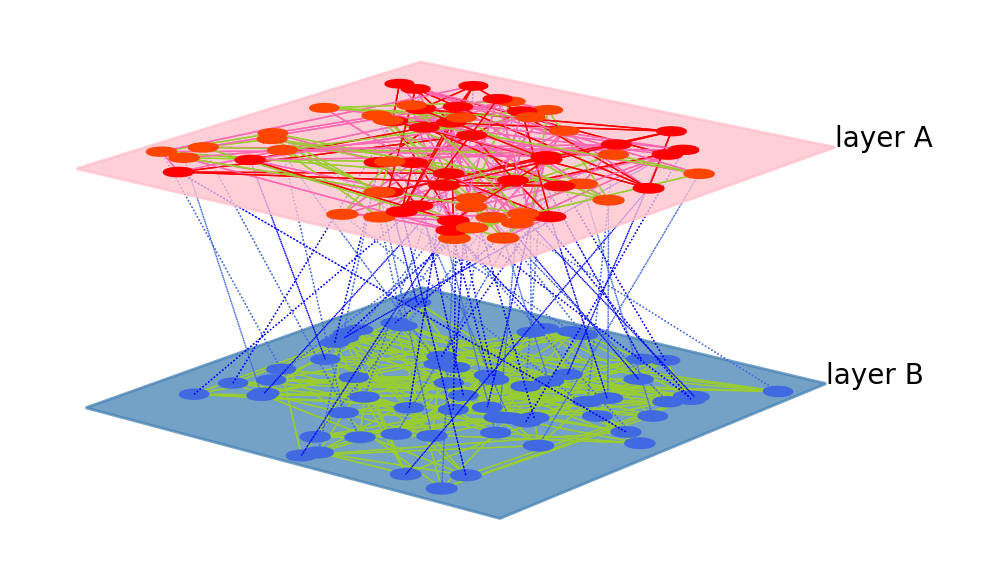
\includegraphics[width=\hsize]{chap3_RR(5)_RR(5).png}
	\caption{Competition on random regular network}
	\label{chap3_RR(5)_RR(5)}
\end{figure}
\begin{figure}[!htb]
	\centering
	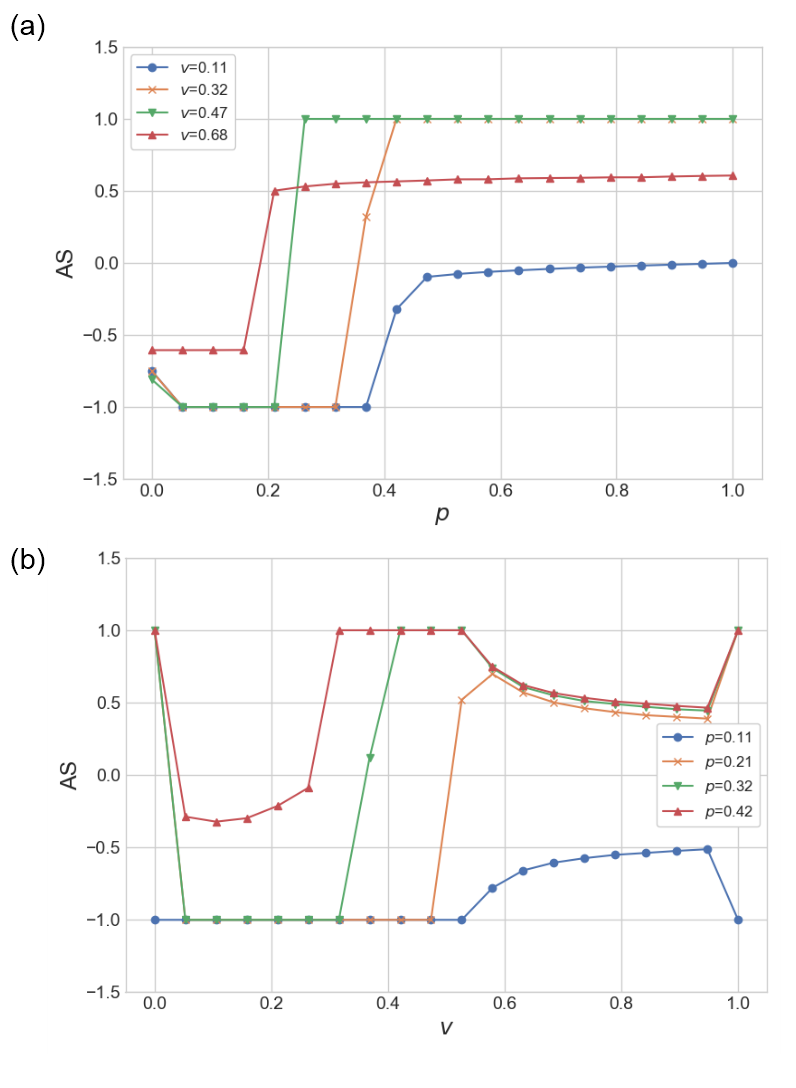
\includegraphics[width=\hsize]{chap3_RR(5)_RR(5)_2d.png}
	\caption{(a) $p$-\textit{AS} chart according to specific $v$ values. (b) $v$-\textit{AS} chart according to specific $p$ values.}
	\label{chap3_RR(5)_RR(5)_2d}
\end{figure}
\begin{figure}[!htb]
	\centering
	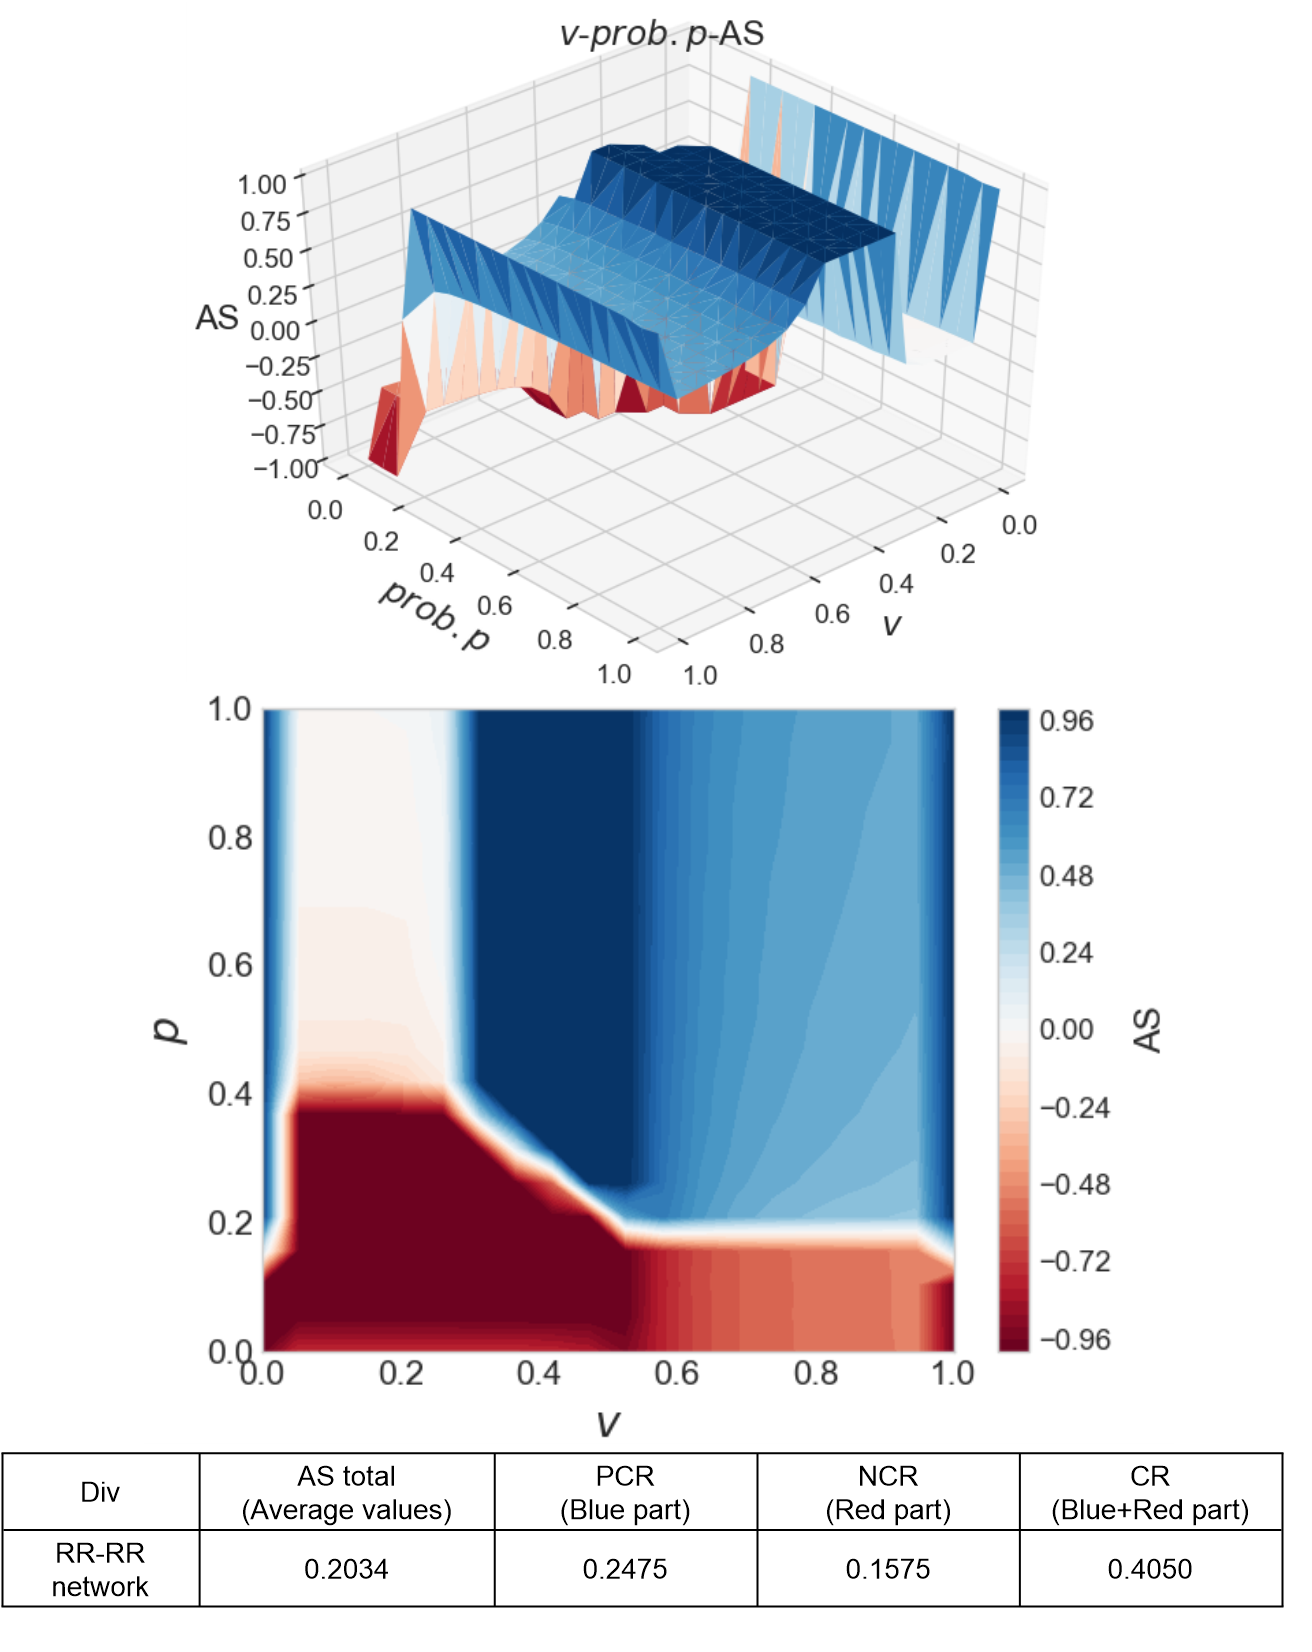
\includegraphics[width=\hsize]{chap3_RR(5)_RR(5)_total.png}
	\caption{\textit{AS} according to all $p$s and $v$s}
	\label{chap3_RR(5)_RR(5)_total}
\end{figure}
In this section, simulation results on a two-layer network with random regular networks are provided to analyze the competition of two layers. Each layer consists of a random regular network that has $N$ nodes with $k$ internal edges as introduced in \parencite{kimsangwoo2012, choi2011, bela2001}. Each node of one layer is connected with a random node on the other layer. That means each node has only one external edge. Simulations are performed on the two-layer network with $N=2048$ and $k=5$ on each layer.

The simulation results are shown in Fig.~\ref{chap3_RR(5)_RR(5)_2d} and Fig.~\ref{chap3_RR(5)_RR(5)_total}.  Fig.~\ref{chap3_RR(5)_RR(5)_2d} presents how the `Average State'(\textit{AS}) is changed according to the other parameter($v$ or $p$) when one parameter($p$ or $v$) is constant. So we can know how each parameter works on the network. Fig.~\ref{chap3_RR(5)_RR(5)_total} provides total results with all parameters. Through these figures, the characteristics of the network are analyzed.

Fig.~\ref{chap3_RR(5)_RR(5)_2d}(a) shows that when $p > 0.2$, $0.32 < v < 0.47$, it normally tends to have positive consensus. We find that if $v$ is lower or larger than a certain value, it does not make consensus. In Fig.~\ref{chap3_RR(5)_RR(5)_2d}(b), as $v$ increases, it normally changes from negative to positive consensus. However, it is found out that when $p$ is small enough($p \le 0.11$), it does not make a positive consensus.  To sum up, when $p$ is large enough, it tends to make a positive consensus. However, when $v$ is small enough, it tends to be changed into a negative consensus.

Fig.~\ref{chap3_RR(5)_RR(5)_total} shows the states of two layers according to all $p$s and all $v$s. As previously described in the chapter.\ref{chap2}, blue areas are for positive consensus, red areas are for negative consensus, and light-colored and white areas are for coexistence. Moreover, indexes for consensus are also measured. \textit{PCR} value is $0.2475$, and \textit{NCR} value is $0.1575$. The ratio of coexistence is $1 - CR = 0.5950$. By using these values and figures, this model is compared with networks of various structures in the next section. Through these figures, the characteristics of parameters can be arranged as follows: First, large $p$ tends to make positive consensus, and small $p$ tends to make negative consensus. Second, small $v$ tends to make negative consensus, and large $v$ tends to make coexistence state. \\

\section{Competition on Networks with different number of external links}
\begin{figure}[!htb]
	\centering
	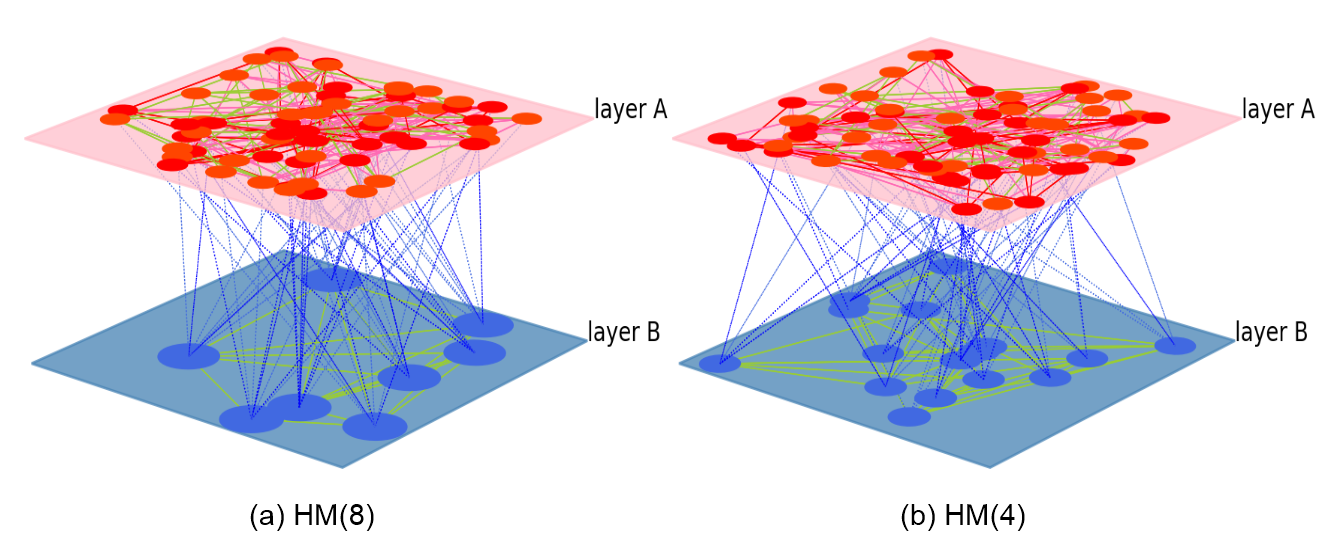
\includegraphics[width=\hsize]{chap3_HM.png}
	\caption{Competition on \textit{Hierarchical Model}}
	\label{chap3_HM}
\end{figure}
In this section, we consider the influence of external links. Based on the \textit{RR-RR} model in section.~\ref{competition on Random Regular Networks}, we reduce the number of nodes in layer B at a specific rate and increase the external links from nodes in layer B accordingly, as shown in Fig.~\ref{chap3_HM}.  We denote \textit{HM(n)} as a \textit{Hierarchical Model} with a level $n$, which means that the number of nodes in layer B is $1/n$ of the number of nodes in layer A, and the number of external links from a node in layer B is $n$ in view that the number of external links from a node in layer A is $1$. In other words, each node in layer A has one external edge, but each node in layer B has $n$ external edges for \textit{HM(n)}, which means one node in layer B can interact with $n$ nodes in layer A.

\begin{figure}[!htb]
	\centering
	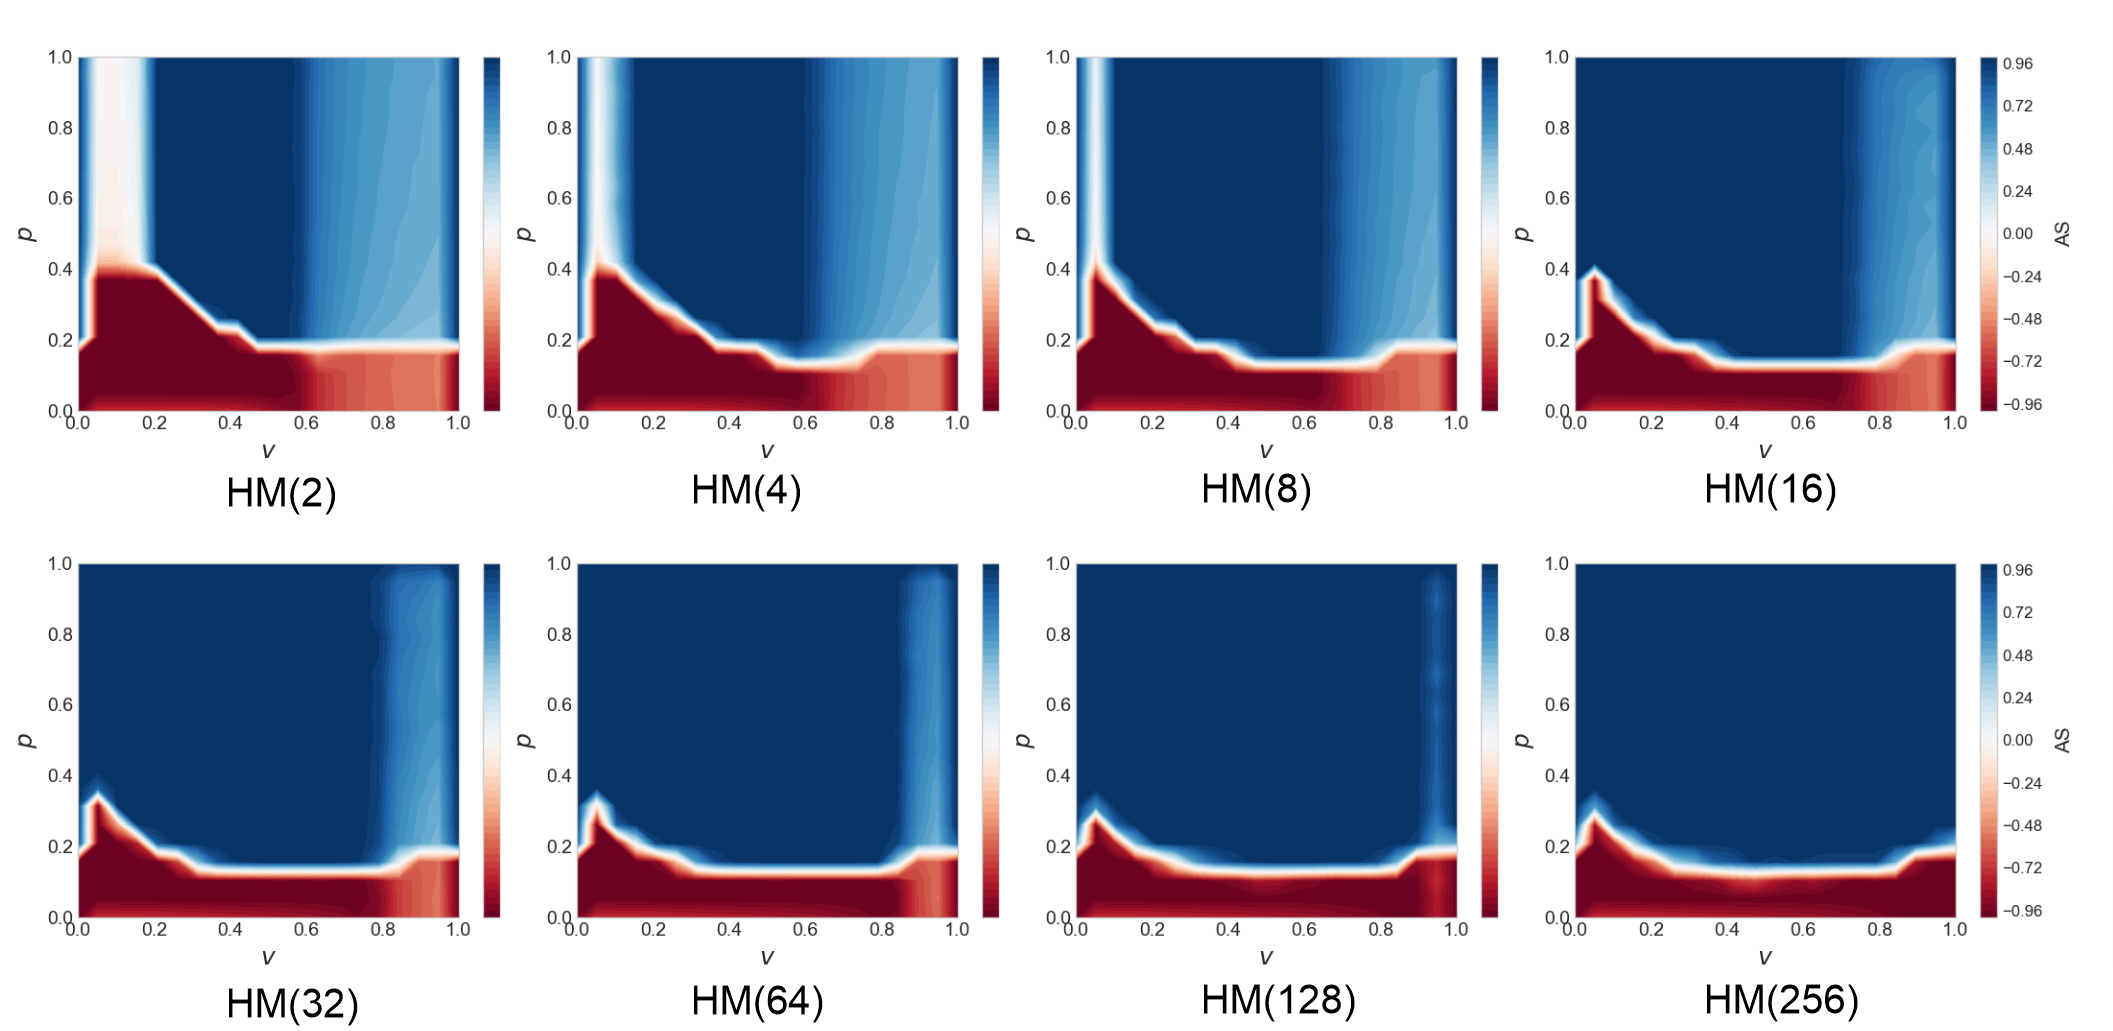
\includegraphics[width=\hsize]{chap3_HMs_AStotal.png}
	\caption{\textit{AS total} on various \textit{Hierarchical Models}}
	\label{chap3_HMs_AStotal}
\end{figure}

Various \textit{HM(n)s} are simulated.  The simulation results of $8$ \textit{HM(n)}s, \textit{HM(2), HM(4), HM(8), HM(16), HM(32), HM(64), HM(128), HM(256)} are arranged, as shown in Fig.~\ref{chap3_HMs_AStotal}. Fig.~\ref{chap3_HMs_AStotal} shows that \textit{HM(2)} has the most significant area for the coexistence part(light-colored and white area), and \textit{HM(256)} has the most significant area for the consensus part(blue and red area). As $n$ in \textit{HM(n)} is increased, the coexistence area is decreased, and the consensus area is increased. Notably, the positive consensus area is significantly increased, the negative consensus area is slightly decreased.
 
\begin{figure}[!htb]
	\centering
	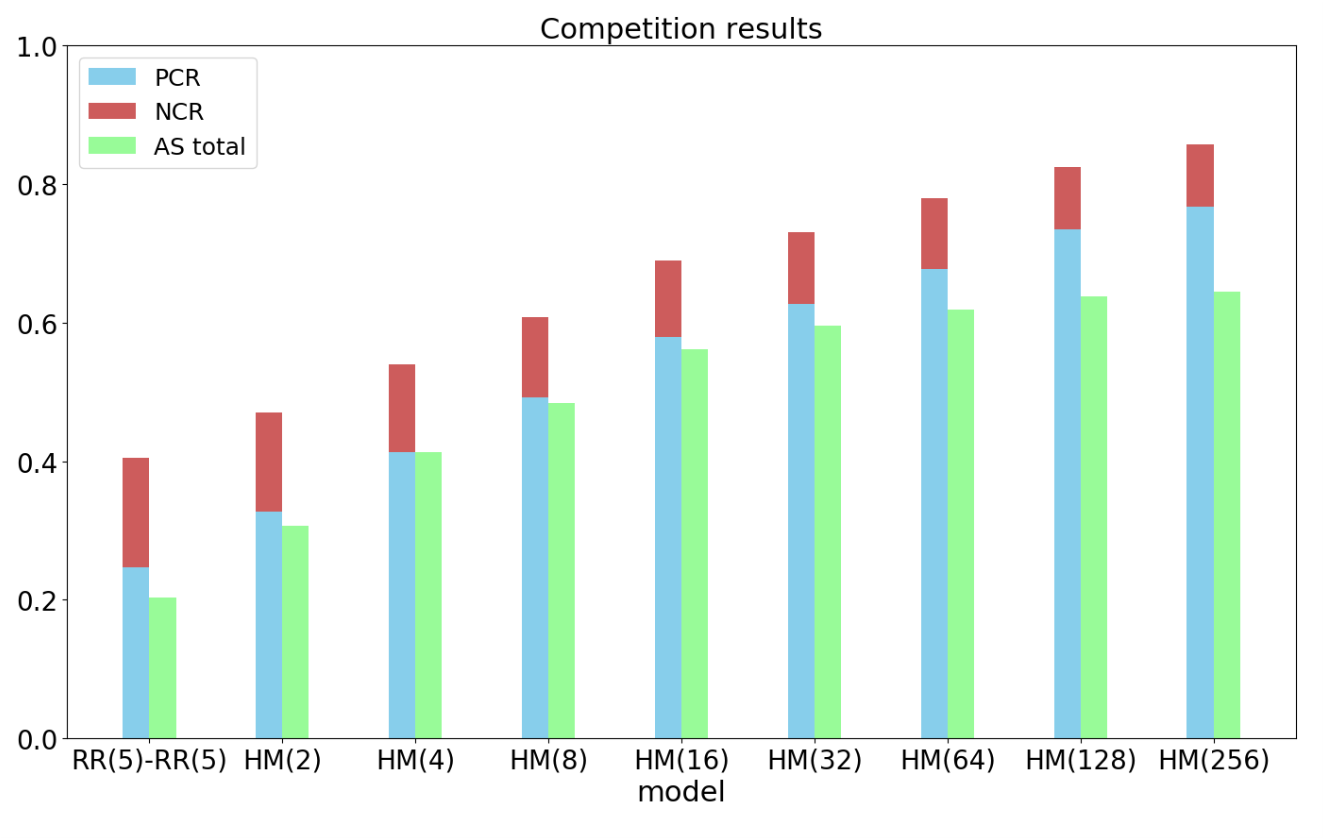
\includegraphics[width=\hsize]{chap3_HMs_total.png}
	\caption{Histogram for \textit{PCR, NCR, AS total} of \textit{Hierarchical Models(HM(n))}}
	\label{chap3_HMs_total}
\end{figure}

To find out the difference between models, we use the indexes, \textit{PCR, NCR, AS total}. Fig.~\ref{chap3_HMs_total} shows the results to analyze \textit{HM(n)} with indexes. The blue color bar is for \text{PCR}, the red color bar is for \text{NCR}, and the green color bar is for \text{AS total}. Comparing \textit{HMs} with the \textit{Basic model(RR(5)-RR(5))}, \textit{CR} \textit{PCR}, and \textit{AS total} are all increased remarkably. \textit{HMs} have a larger area for positive consensus than \textit{RR(5)-RR(5)}. Moreover, \textit{HMs} have a smaller area for negative consensus than \textit{RR(5)-RR(5)}. 

In summary, all the \textit{Hierarchical Model} has more massive \textit{CR} than \textit{Random Regular Network}. However, \textit{PCR} is increased, but \textit{NCR} is decreased. It is found out that as the number of nodes in layer B is decreased as a larger ratio, the network makes it easier to have a positive consensus and harder to have a negative consensus. In the real world, it can be analyzed that as the number of leaders is much smaller, social conflict is decreased, and the opinion is convergent to social opinion(layer A). However, sometimes there are some dangers to ignore the leader opinions(layer B), or to cause more social conflicts when there are stubborn leaders; that case is simulated in the chapter.\ref{chap5}. \\

\section{Competition on Networks with different number of internal links}

\begin{figure}[!htb]
	\centering
	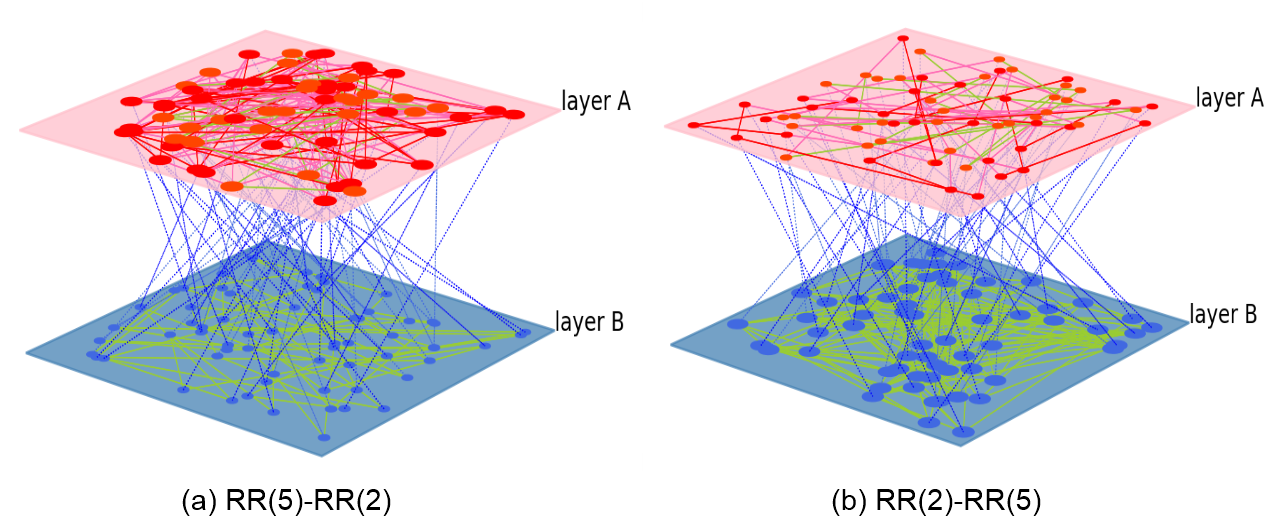
\includegraphics[width=\hsize]{chap3_changing_internal_edges.png}
	\caption{Competition on interconnected networks with different internal edges}
	\label{chap3_changing_internal_edges}
\end{figure}

Next, the interconnected networks are simulated with various internal degrees in order to define and evaluate the influence of internal degrees. The random regular network is applied, and the internal degrees on each node is switched to various numbers, as shown in Fig.~\ref{chap3_changing_internal_edges}. However, there is no change in external degree, which is fixed to only $1$. Here, \textit{RR(n)-RR(m)} represents layer A has a random regular network with $n$ internal edges per node, and layer B has a random regular network with $m$ internal edges per node.

\begin{figure}[!htb]
	\centering
	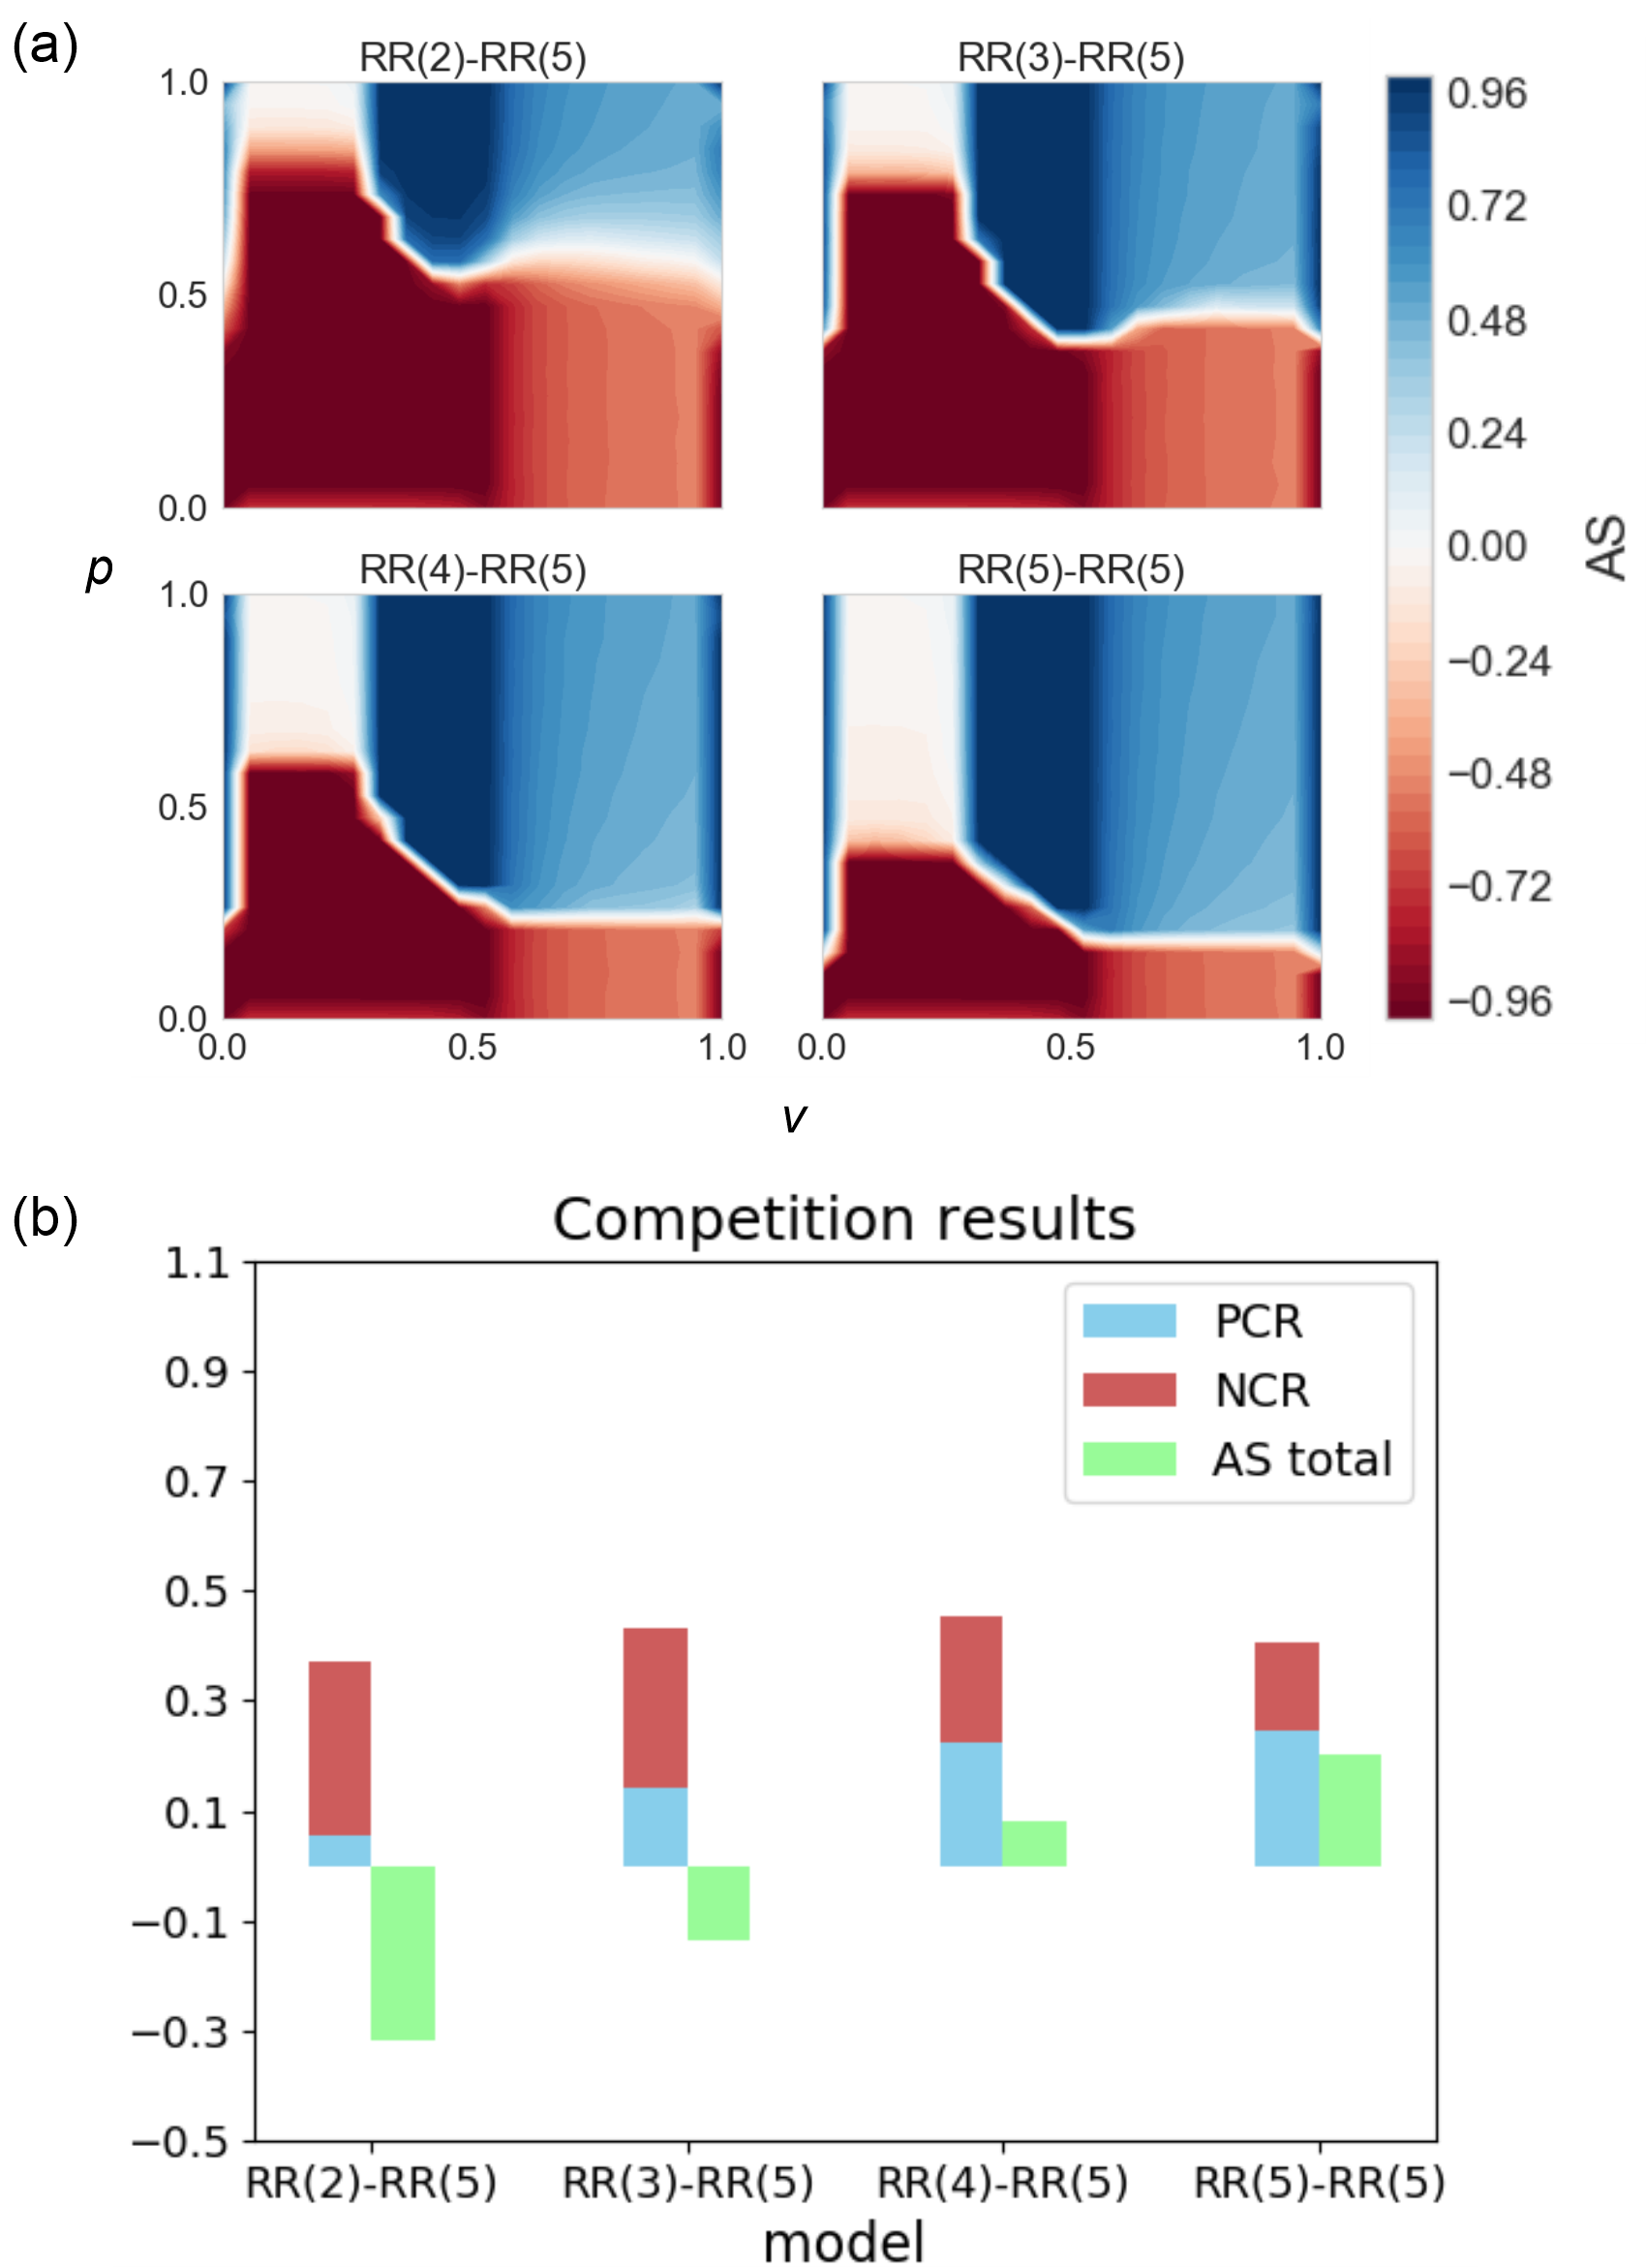
\includegraphics[width=\hsize]{chap3_internal_edge_A_total1.png}
	\caption{Simulation results with different internal degrees on layer A}
	\label{chap3_internal_edge_A_total}
\end{figure}

First, the internal degrees on layer A is changed. The internal degree on layer B is fixed to $5,120$, which means each node has $5$ internal edges on layer B, and the internal degree on layer A is switched into $2,048$, $3,072$, $4,096$, or $5,120$, which means each node has $2$, $3$, $4$, or $5$ internal edges on layer A. Fig.~\ref{chap3_internal_edge_A_total} shows the simulation results according to changing the internal degree on layer A. As shown in Fig.~\ref{chap3_internal_edge_A_total} (a), as the internal degree on layer A is increased, the red area is decreased, and the blue area is increased. Moreover, the results are presented with the indexes, \textit{PCR, NCR, AS total} in Fig.~\ref{chap3_internal_edge_A_total} (b), which shows that as the internal degree on layer A is increased, the negative consensus is decreased, and the positive consensus is increased. As shown in Fig.~\ref{chap3_internal_edge_A_total}, RR(5)-RR(5) has the largest \textit{PCR}, and RR(2)-RR(5) has the largest \text{NCR}. However, all models in Fig.~\ref{chap3_internal_edge_A_total} have almost the same \textit{CR}. It can be analyzed that the internal degree on layer A tends to keep a positive state and to change a negative state into a positive state. 
\begin{figure}[!htb]
	\centering
	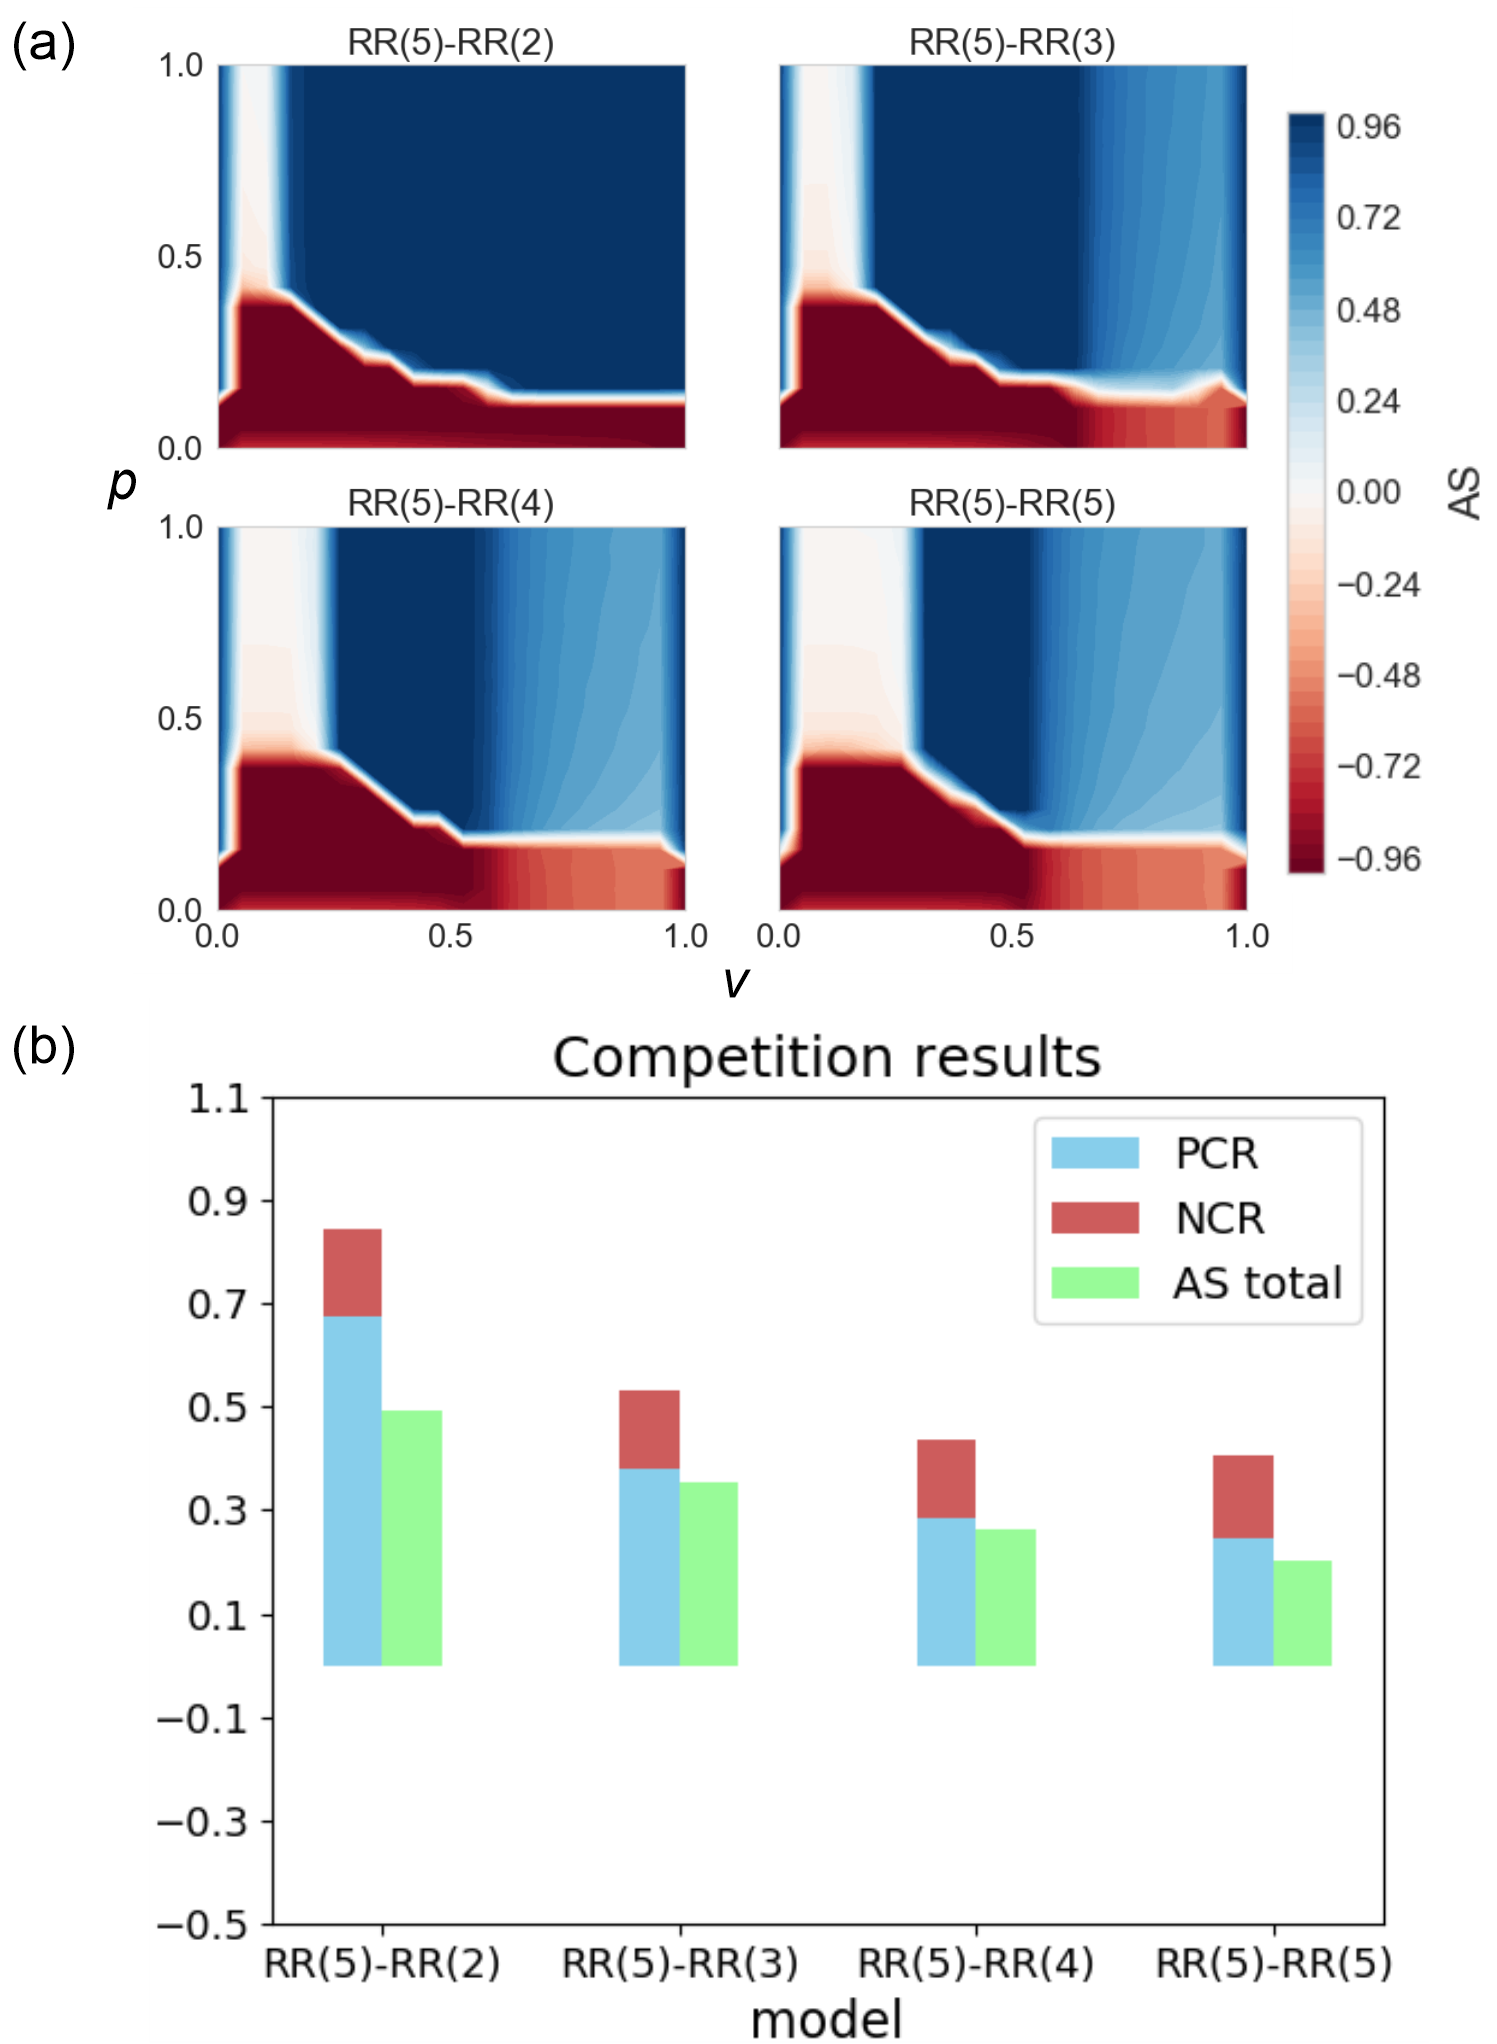
\includegraphics[width=\hsize]{chap3_internal_edge_B_total1.png}
	\caption{Simulation results with different internal degrees on layer B}
	\label{chap3_internal_edge_B_total}
\end{figure}

Next, the internal degree on layer B is switched. The internal degree on layer A is fixed to  $5,120$, which means each node has $5$ internal edges on layer A, and the internal degree on layer B is switched into $2,048$, $3,072$, $4,096$, or $5,120$, which means each node has $2$, $3$, $4$, or $5$ internal edges on layer B. Fig.~\ref{chap3_internal_edge_B_total} shows the results simulated with changing the internal degree on layer B. As shown in Fig.~\ref{chap3_internal_edge_B_total} (a), as the internal degree on layer B is increased, the blue area is decreased, the white and light-colored area is increased, and the red area is almost the same, though the shape of the red area is a little changed.  As shown in Fig.~\ref{chap3_internal_edge_B_total} (b), \textit{RR(5)-RR(2)} has the largest \textit{PCR} and \textit{CR}, and \textit{RR(5)-RR(5)} has the smallest \text{PCR} and \textit{CR}. However, all models in Fig.~\ref{chap3_internal_edge_B_total} have almost the same \textit{NCR}. It can be analyzed that the internal degree on layer B has the tendency to hinder the positive consensus state and has an inverse relation with \textit{CR}. As the internal degrees on layer B is increased, \textit{PCR} and \textit{CR} are inversely decreased.

Considering two cases where an internal degree of layer A is changed and where an internal degree of layer B is changed, it is recognized that the role of internal degree on layer A is different with an internal degree on layer B. The internal degree on layer A has the function to keep the state of layer A and the internal degree on layer B has the function to restrain the consensus state of layer A and make a coexistence state. 

\begin{figure}[!htb]
	\centering
	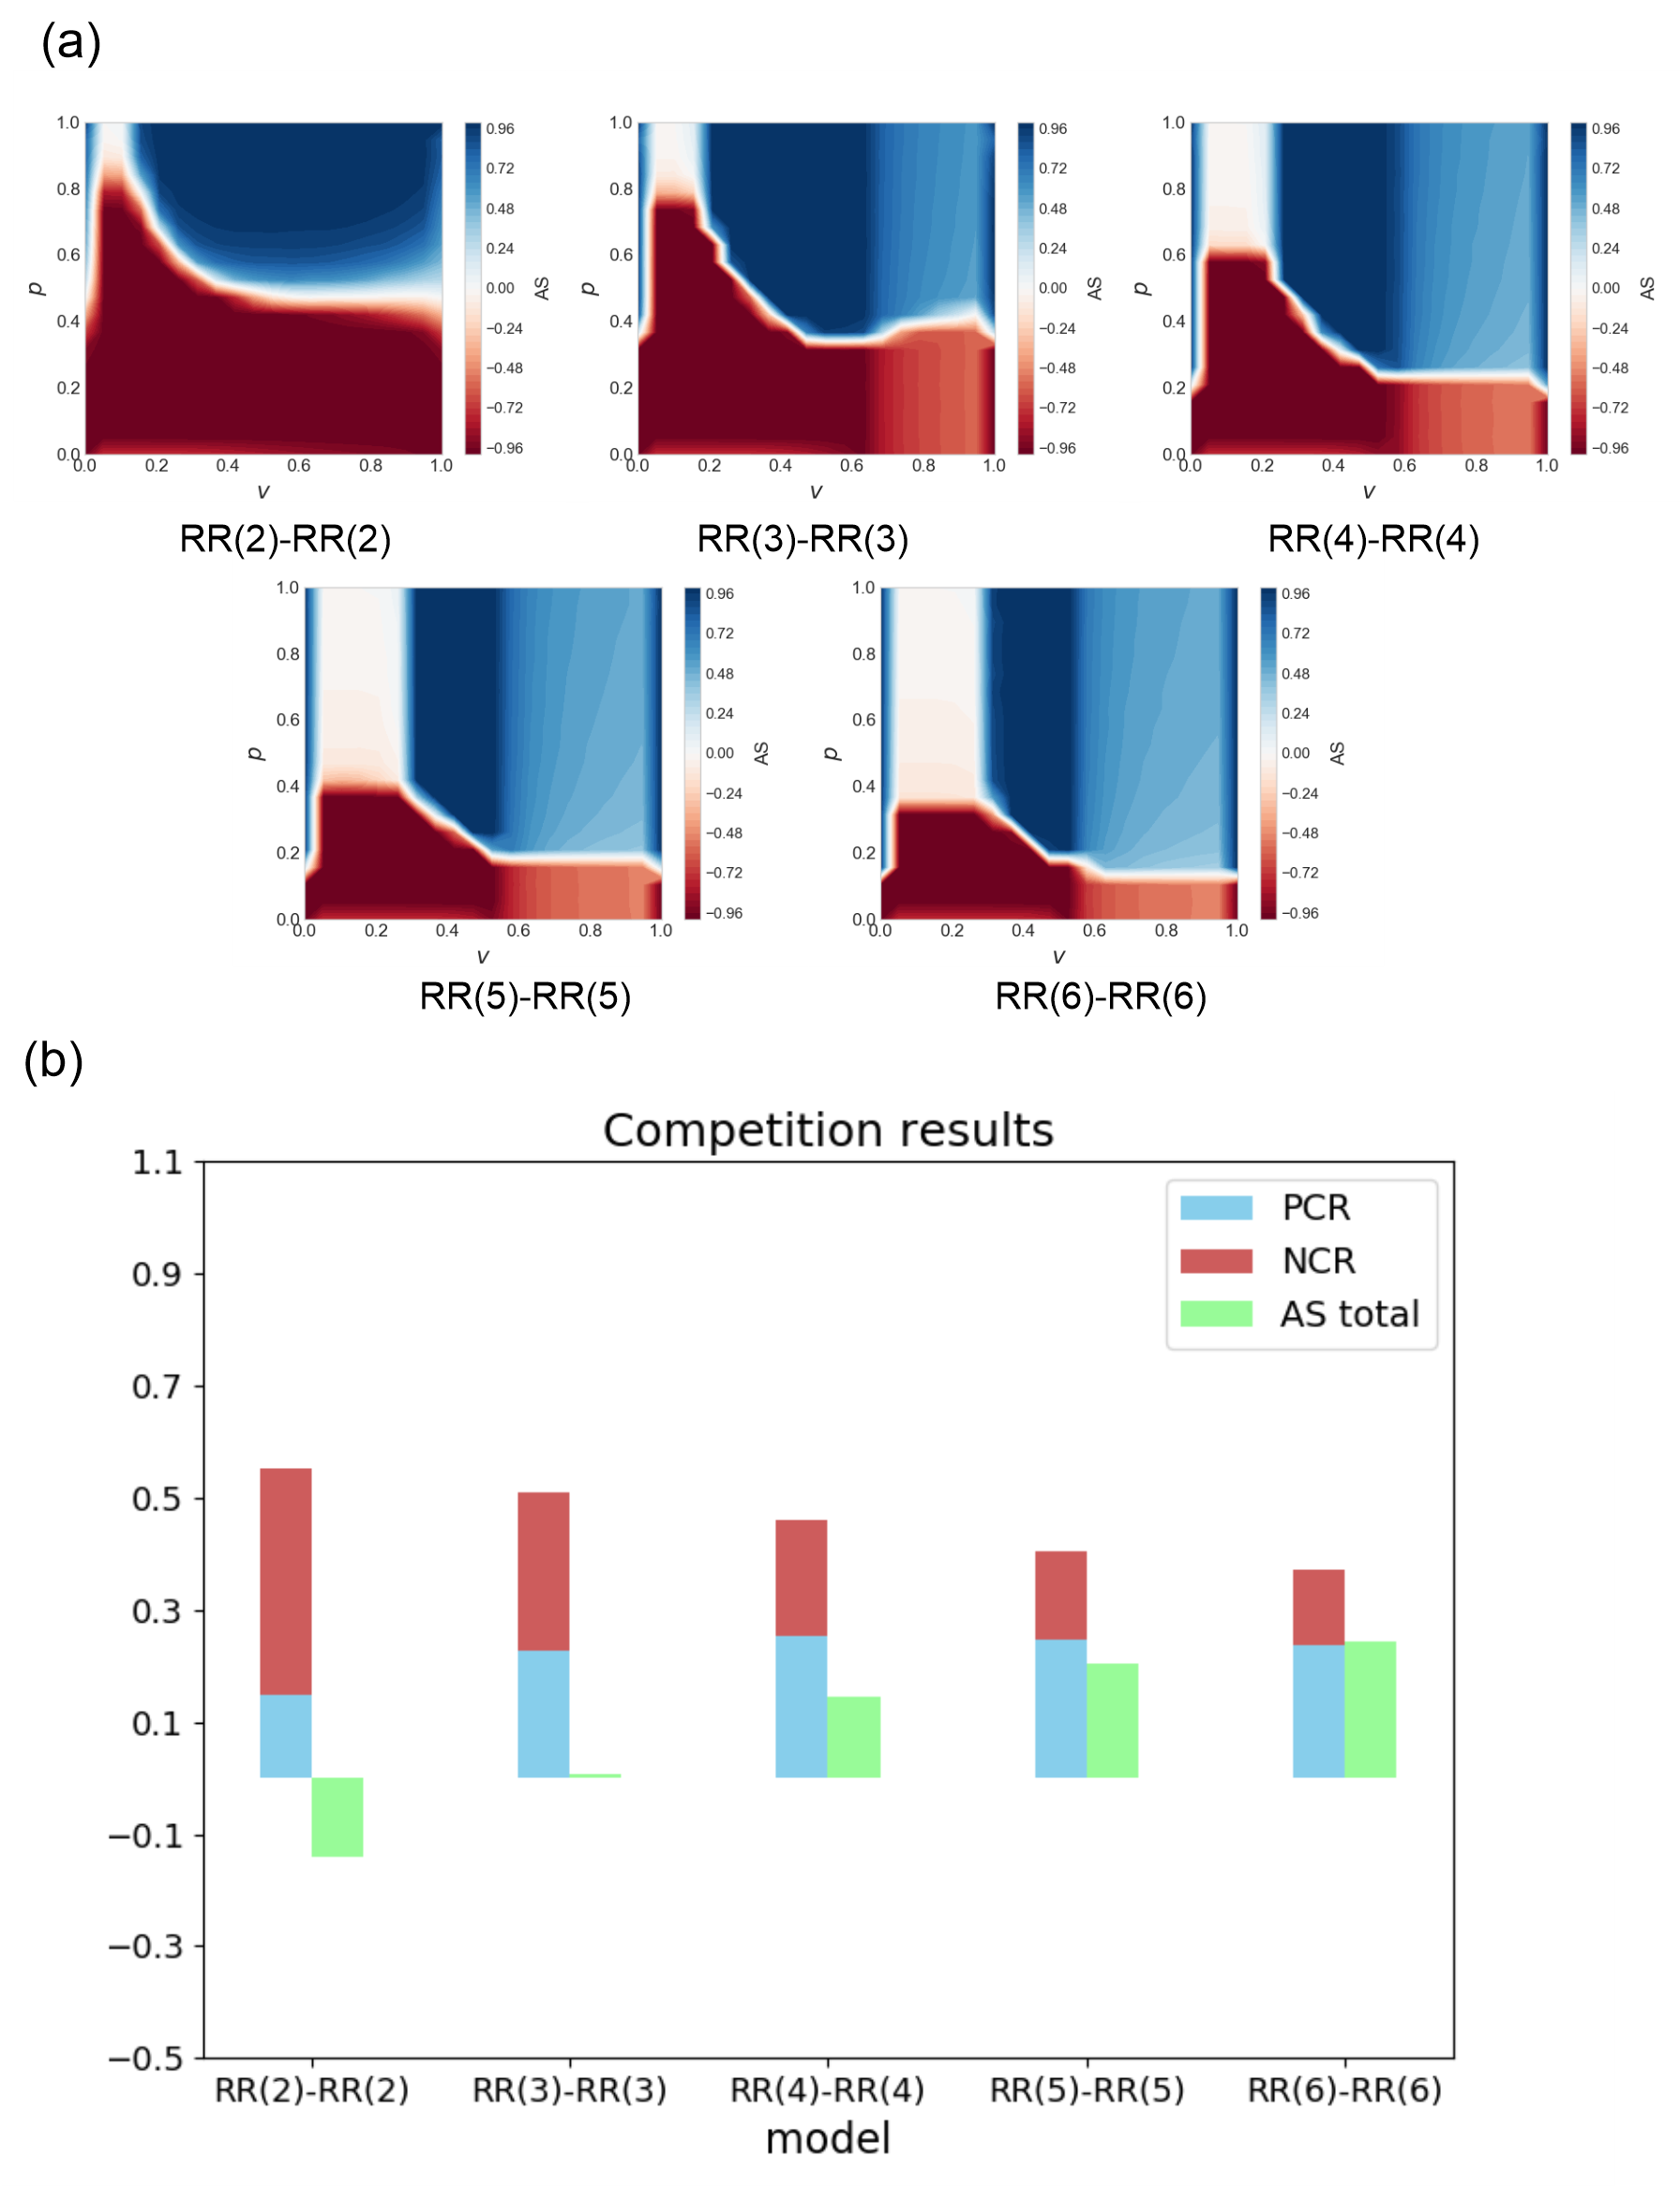
\includegraphics[width=\hsize]{chap3_internal_edge_two_total.png}
	\caption{Simulation results with changing internal degrees on both layers}
	\label{chap3_internal_edge_two_total}
\end{figure}

Next, it is simulated that internal degrees are changed on both layer A and layer B, such as \textit{RR(2)-RR(2), RR(3)-RR(3), RR(4)-RR(4), RR(5)-RR(5)} and \textit{RR(6)-RR(6)}. Through these simulations, it is shown how a total internal degree on both layer A and layer B also affects the state of the interconnected network.

Fig.~\ref{chap3_internal_edge_two_total} shows the influence of a total internal degree on both layers. As the total internal degree is increased, \textit{CR} is inversely decreased, and the ratio of \textit{PCR}(the ratio of the blue bar in a histogram) is increased, but the ratio of \textit{NCR}(the ratio of the red bar in a histogram) is decreased. It can be analyzed that a decrease in \textit{CR} is caused by an increase in internal degree on layer B, and an increase in the ratio of \textit{PCR} is brought out by an increase in internal degree on layer A. But, when the total internal degrees is increased, \textit{PCR, NCR, CR} indexes are decreased. It can be analyzed that a massive internal degree on both layers makes it hard for the state of the network to reach consensus. 
\begin{figure}[!htb]
	\centering
	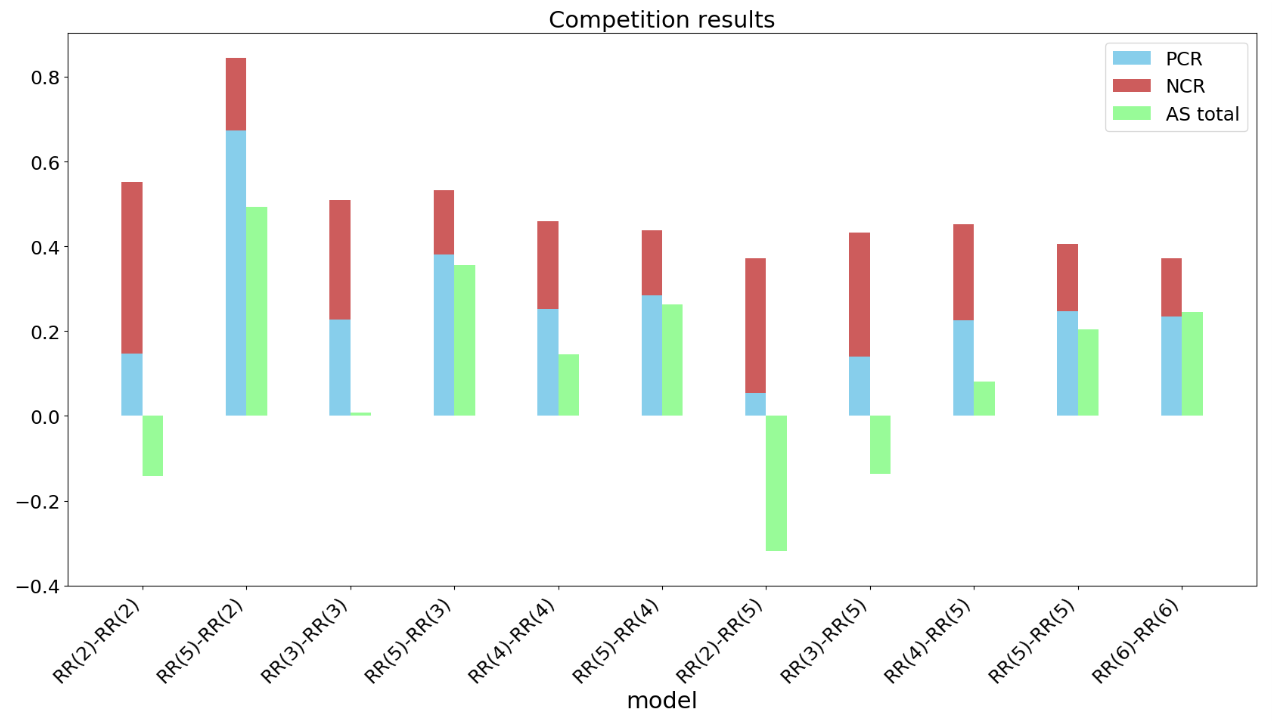
\includegraphics[width=\hsize]{chap3_internal_edge_AB_total.png}
	\caption{Total results with different internal degrees on two layers}
	\label{chap3_internal_edge_AB_total}
\end{figure}

In summary, three main simulations have been implemented to find out the influence of internal degree on an interconnected network by changing the internal degree on layer A, changing the internal degree on layer B and changing the internal degrees on both layers. The results are arranged as follows. First, it is found out that internal degrees on layer A tend to keep a positive state and to change a negative state into a positive state. Second,  it is shown that the number of internal degrees on layer B has the tendency to hinder the positive consensus state and has an inverse relation with \textit{CR}. Third, a massive internal degree makes it hard for the state of the network to reach consensus. 

\begin{figure}[!htb]
	\centering
	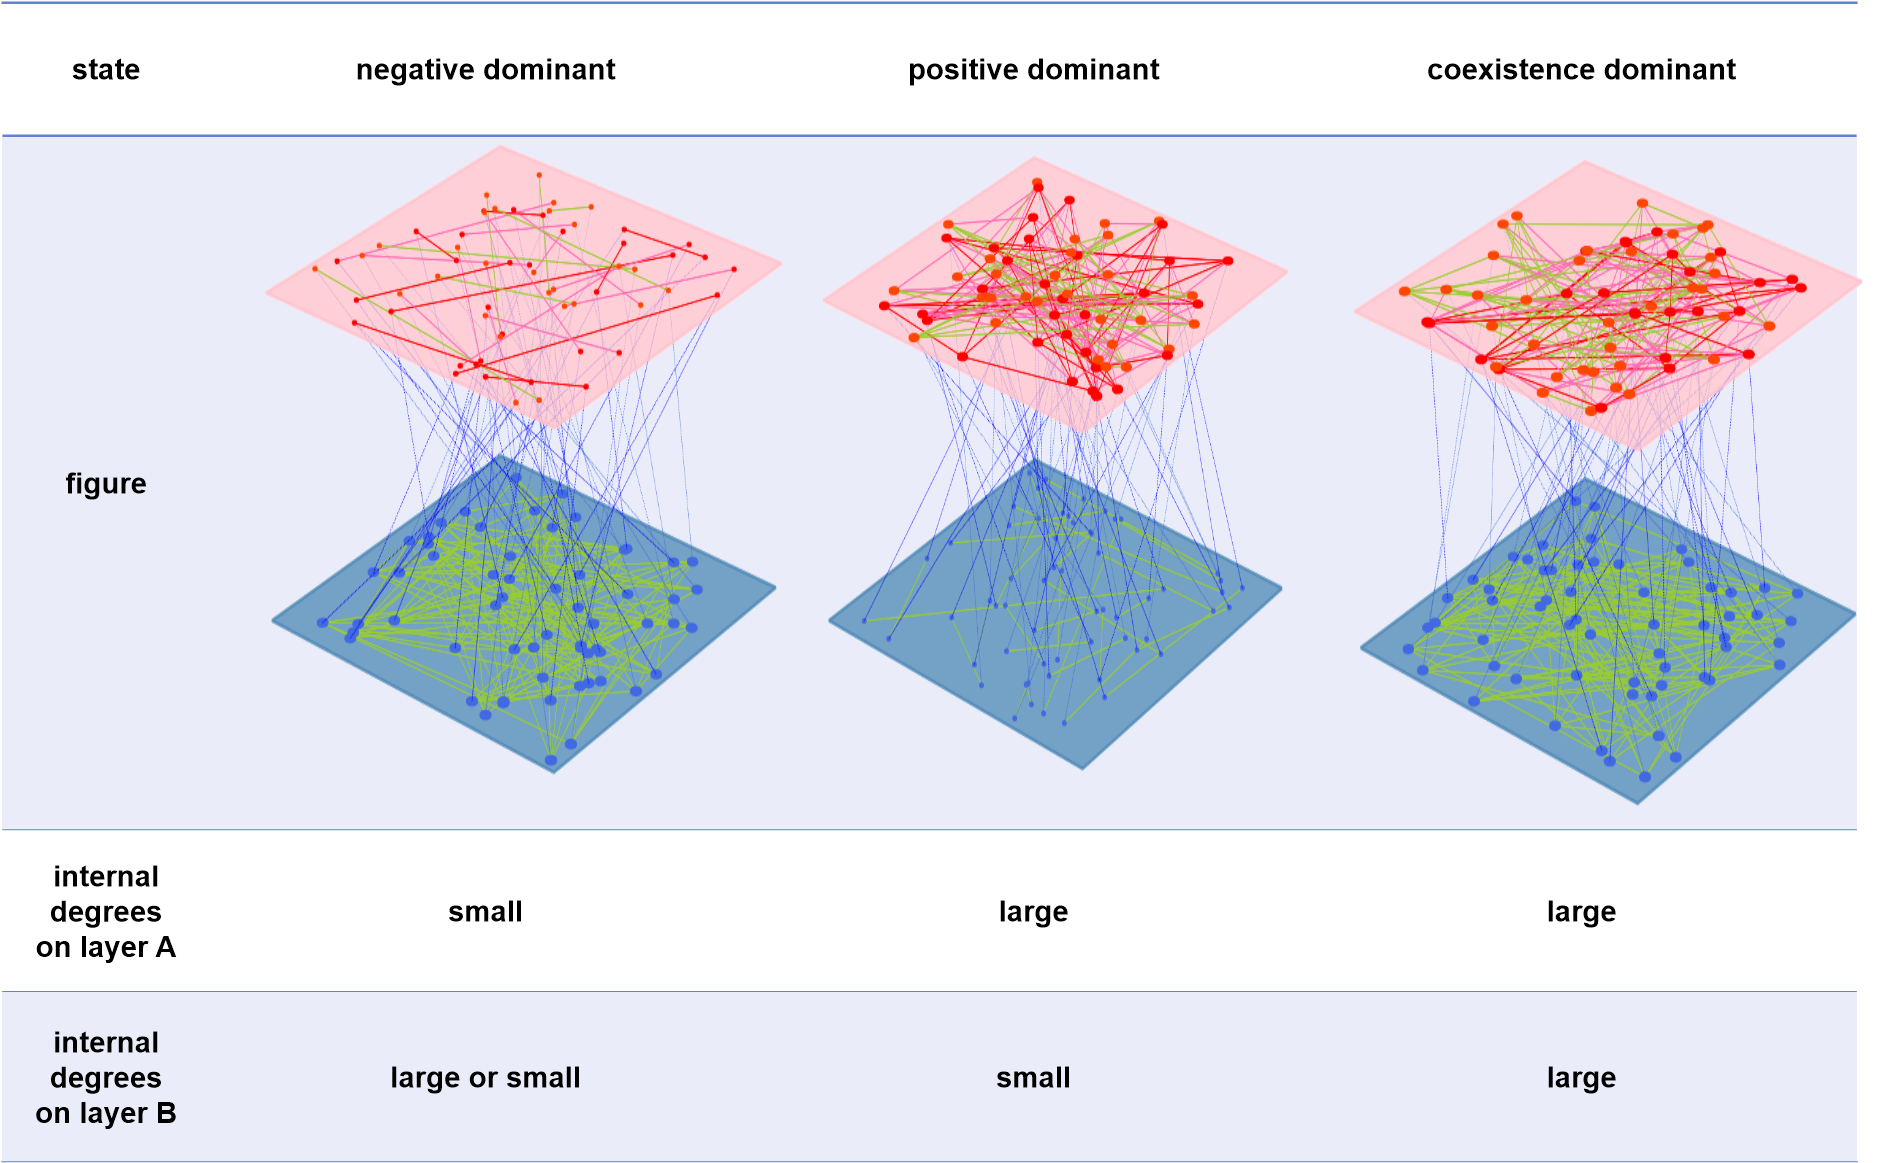
\includegraphics[width=\hsize]{chap3_internal_edge_summary.png}
	\caption{Categorizing the state of the network according to internal degrees on two layers}
	\label{chap3_internal_edge_summary}
\end{figure}

Fig.~\ref{chap3_internal_edge_AB_total} shows the result for all simulations. Through these simulation results, we can analyze how the state of the network is changed according to the internal degrees. Several conclusions can be arranged, as shown in Fig.~\ref{chap3_internal_edge_summary}.  First, it is easy to reach negative consensus(negative dominant) when the internal degrees on layer A is relatively small(the internal degrees on layer B does not matter). Second, it is easy to make positive consensus(positive dominant) when the internal degrees on layer A is relatively large, and the internal degrees on layer B is relatively small. Third, it is easy to make coexistence state(coexistence dominant) when the internal degrees on both layers are too large. \\ 

\section{Competition on Networks with different network structures}
\begin{figure}[!htb]
	\centering
	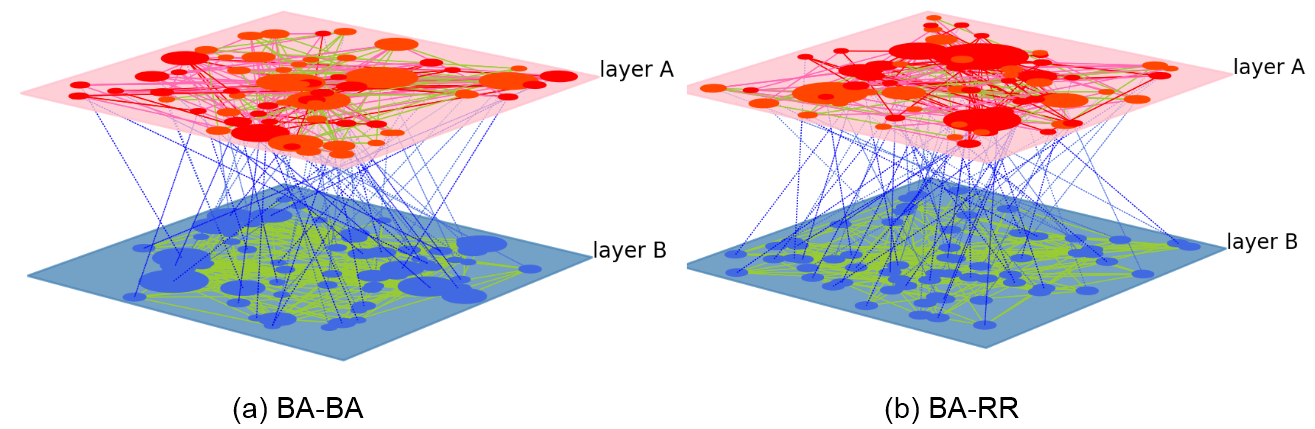
\includegraphics[width=\hsize]{chap3_changing_structure_type.png}
	\caption{Competition on networks with different structures}
	\label{chap3_changing_structure_type}
\end{figure}
So far, the interconnected networks have been simulated with only \textit{RR(random regular networks)} that have the same number of edges for each node. Now, the simulations are implemented on different network types. Here, we use the \textit{Barabasi-Albert network(BA)} structure, as introduced in \parencite{barabasi1999}. \textit{Barabasi-Albert(BA)} network has $N$ nodes with attaching new nodes, each with $K$ edges that are preferentially attached to existing nodes with high degrees. However, there is no change in the external degree, which is fixed to only $1$.

\begin{figure}[!htb]
	\centering
	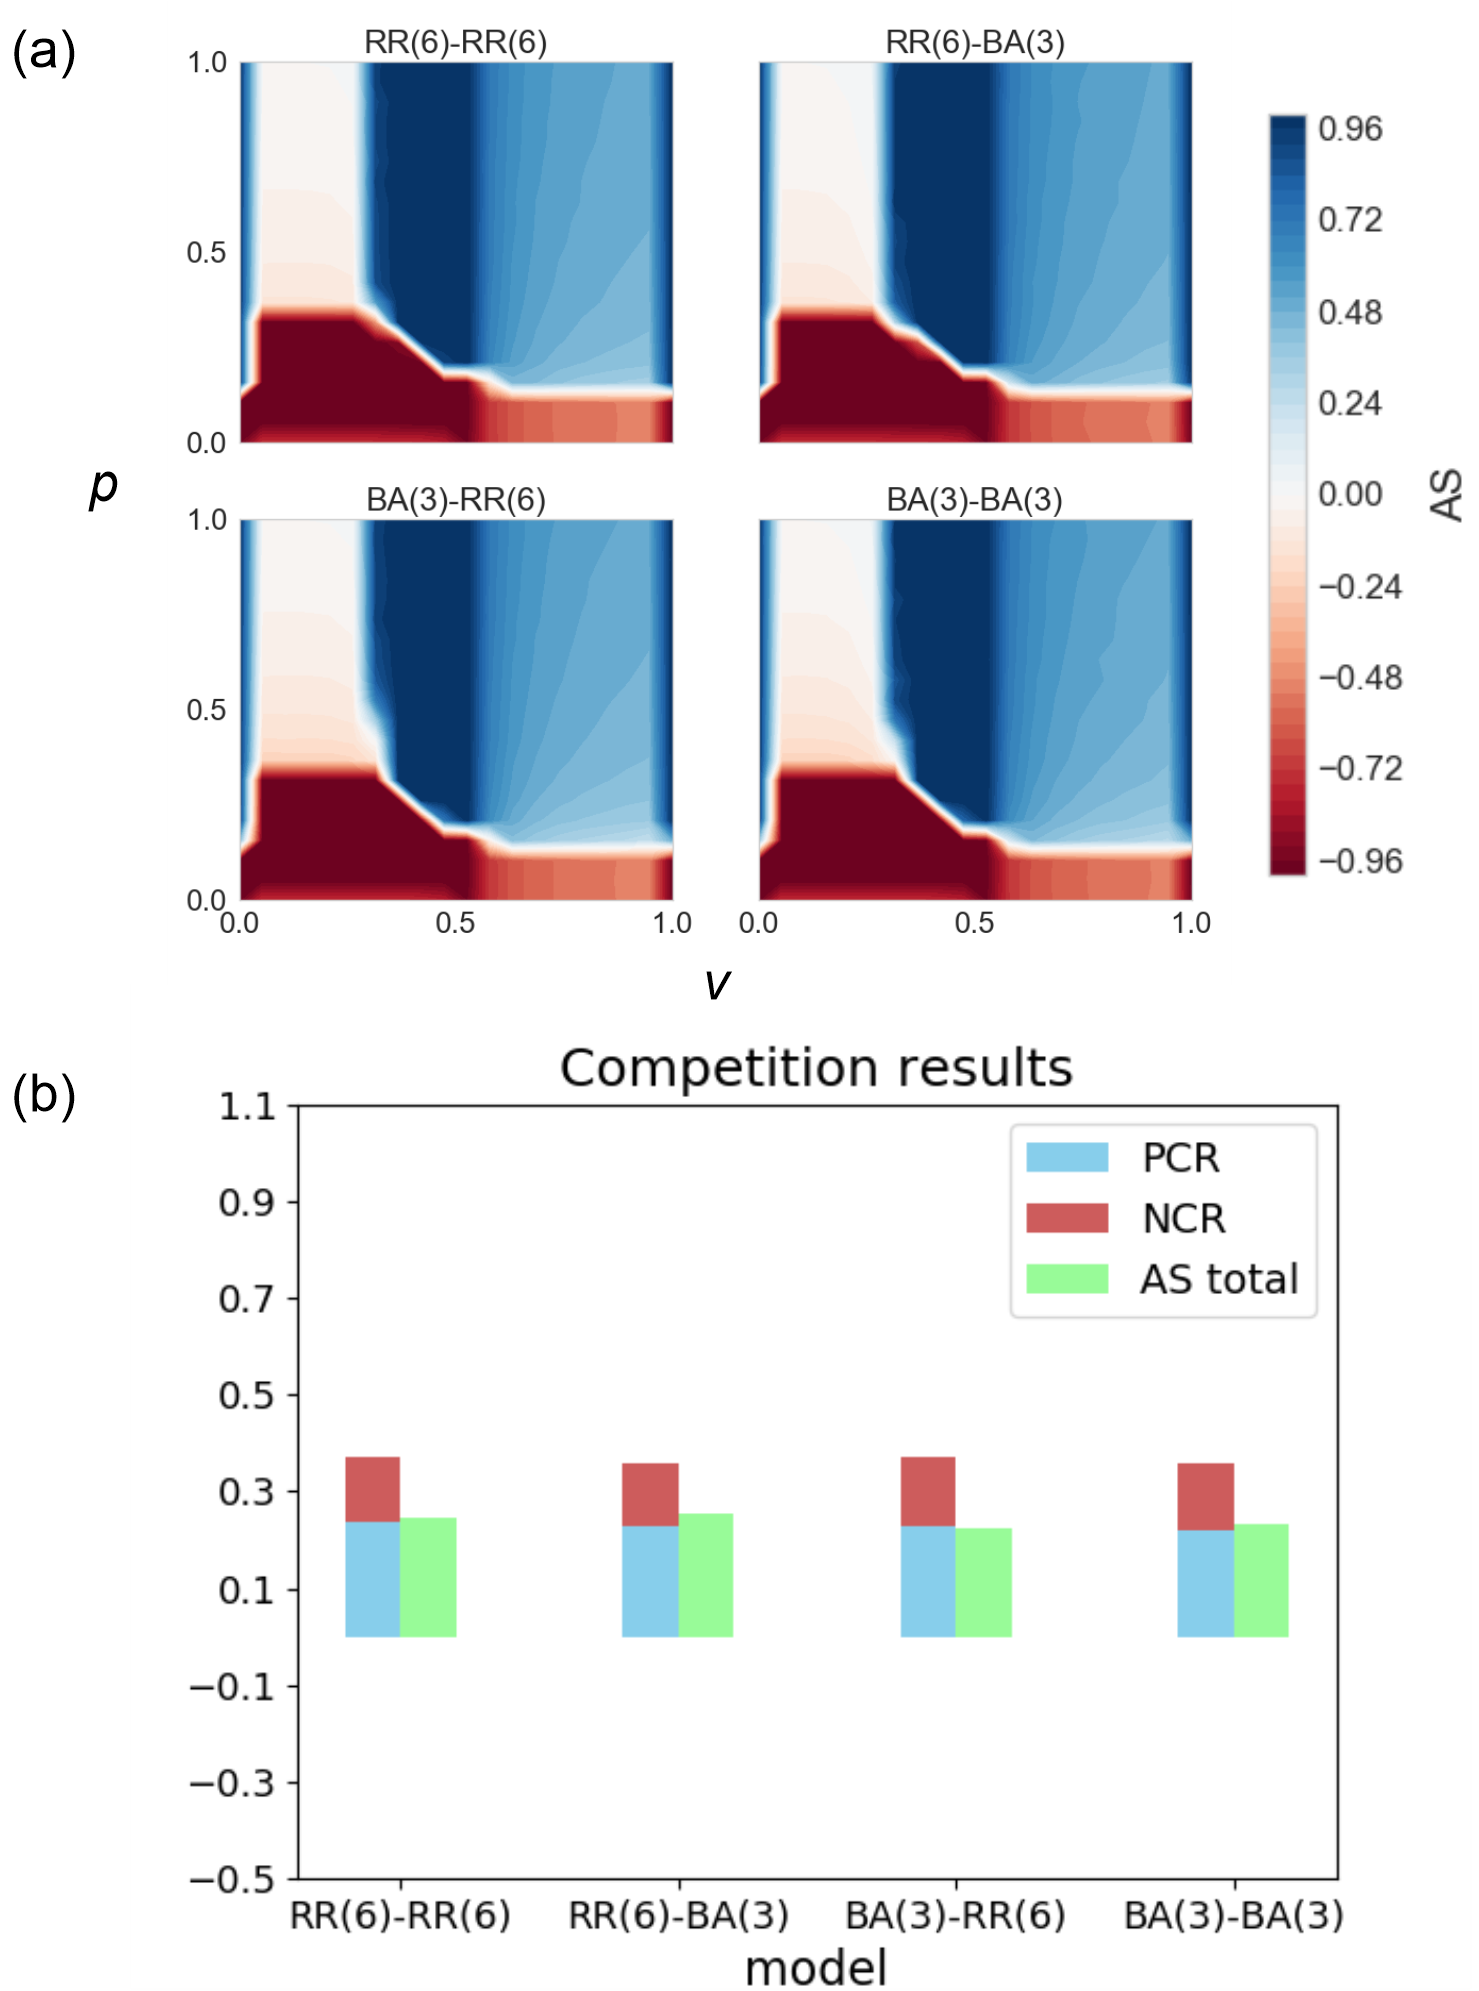
\includegraphics[width=\hsize]{chap3_changing_network_type11.png}
	\caption{Simulation results with different network types}
	\label{chap3_changing_network_type1}
\end{figure}

Four simulations are implemented with switching network structures. The \textit{BA} or \textit{RR} network is applied for both layers or switched on each layer. In order to restrain the influence of an internal degree, the number of internal edges in \textit{BA} is set up to be similar to the number of internal edges in \textit{RR}. So, simulations are implemented with $K=6$ on the \textit{RR} network and $K=3$ on the \textit{BA} network. The number of internal edges in the \textit{BA} is $6,135$, and the number of internal edges in the \textit{RR} is $6,144$.

\begin{figure}[!htb]
	\centering
	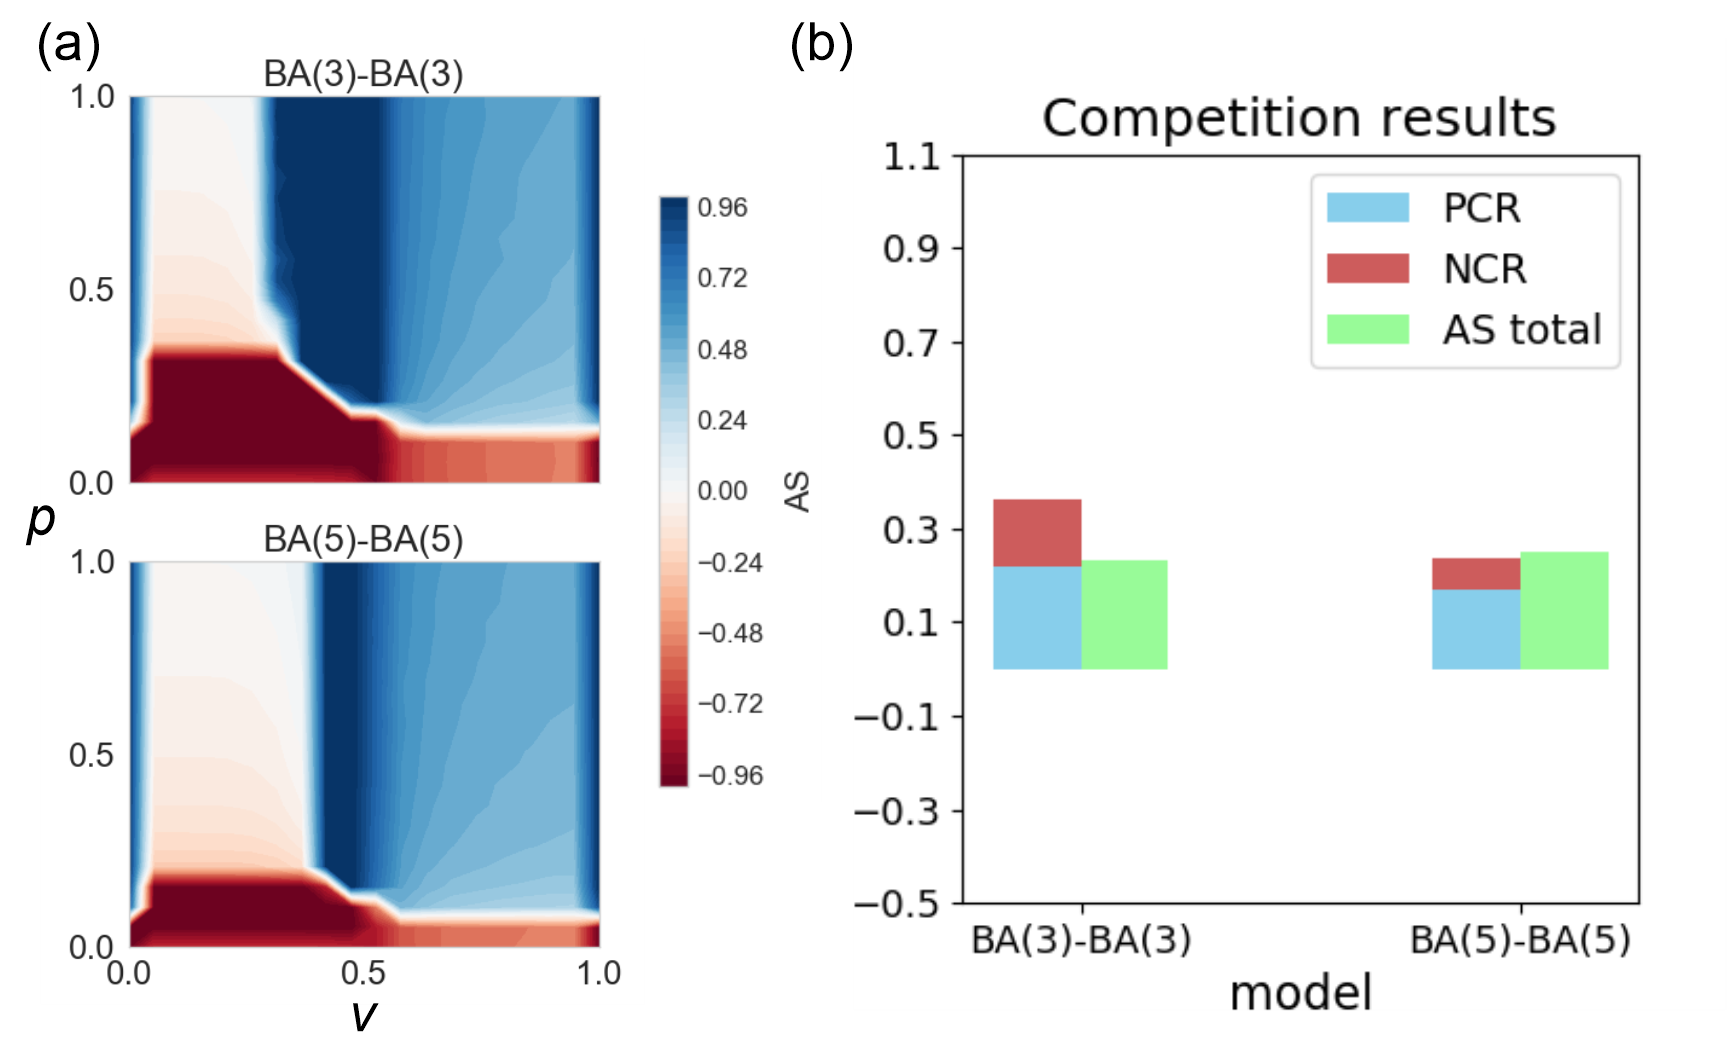
\includegraphics[width=\hsize]{chap3_changing_network_type2.png}
	\caption{Simulation results of BA-BA networks with different internal degrees}
	\label{chap3_changing_network_type2}
\end{figure}

The simulation results are shown in Fig.~\ref{chap3_changing_network_type1}. The results of all simulations have almost the same features. The \textit{PCR, NCR,} and \textit{CR} gaps between simulation results are less than $0.02$ individually. The structure of the network makes no noticeable difference in consensus results. 

Next, the number of internal edges is increased on the network, where it consists of two \textit{BA} networks. It is found out how the number of internal edges works on the different network types with the \textit{RR} network. Two models, \textit{BA(3)-BA(3)} and \textit{BA(5)-BA(5)}, are simulated. \textit{BA(3)-BA(3)} model has $6,135$ internal edges on each layer, and \textit{BA(5)-BA(5)} model has $10,215$ internal edges on each layer.

As shown in Fig.~\ref{chap3_changing_network_type2}, \textit{BA(5)-BA(5)} has a larger coexistence area than \textit{BA(3)-BA(3)} because of too many internal edges. It is shown that the influence of internal degree is more important for changing the state of the network and making consensus than the influence of network type. However, if there are stubborn nodes, which are nodes whose states are fixed during the evolution of opinion, on the networks, the simulation results are different because the centralities of stubborn nodes are changed according to network types. Key nodes selection by using stubborn nodes is simulated and analyzed in chapter.\ref{chap5}.\\

\section{Conclusion}
Various simulations are simulated to find out the role of internal and external degrees and the influence of network types. All results of the simulations are shown in Table.~\ref{Consensus properties of Simulation Models}.
 
\begin{table}[!htb]
	\centering
    \caption{Consensus properties of simulation models}
	\label{Consensus properties of Simulation Models}
	\begin{center}
		\begin{tabular}{c|c|c|c|c|c|c|c|c} \hline\hline
			Div                    & A nodes& B nodes & A edges & B edges & AS total  & PCR    & NCR    & CR       \\ \hline \hline
			RR(2)-RR(5)            & 2,048  & 2,048   & 2,048   & 5,120   & -0.3186   & 0.0550 & 0.3175 & 0.3725   \\ \hline
			RR(3)-RR(5)            & 2,048  & 2,048   & 3,072   & 5,120   & -0.1368   & 0.1400 & 0.2925 & 0.4325   \\ \hline
			RR(4)-RR(5)            & 2,048  & 2,048   & 4,096   & 5,120   &  0.0804   & 0.2250 & 0.2275 & 0.4525   \\ \hline
			RR(5)-RR(2)            & 2,048 	& 2,048   & 5,120   & 2,048   &  0.4927   & 0.6725 & 0.1725 & 0.8450   \\ \hline	
			RR(5)-RR(3)            & 2,048 	& 2,048   & 5,120   & 3,072   &  0.3555   & 0.3800 & 0.1525 & 0.5325   \\ \hline
			RR(5)-RR(4)            & 2,048  & 2,048   & 5,120   & 4,096   &  0.2633   & 0.2850 & 0.1525 & 0.4375   \\ \hline
			RR(2)-RR(2)            & 2,048  & 2,048   & 2,048   & 2,048   & -0.1412   & 0.1475 & 0.4050 & 0.5525   \\ \hline
			RR(3)-RR(3)            & 2,048  & 2,048   & 3,072   & 3,072   &  0.0084   & 0.2275 & 0.2825 & 0.5100   \\ \hline
			RR(4)-RR(4)            & 2,048  & 2,048   & 4,096   & 4,096   &  0.1448   & 0.2525 & 0.2075 & 0.4600   \\ \hline
			RR(5)-RR(5)            & 2,048  & 2,048   & 5,120   & 5,120   &  0.2034   & 0.2475 & 0.1575 & 0.4050   \\ \hline
			RR(6)-RR(6)            & 2,048  & 2,048   & 6,144   & 6,144   &  0.2444   & 0.2350 & 0.1375 & 0.3725   \\ \hline
			RR(6)-BA(3)            & 2,048 	& 2,048   & 6,144   & 6,135   &  0.2541   & 0.2275 & 0.1300 & 0.3575   \\ \hline 
			BA(3)-RR(6)            & 2,048 	& 2,048   & 6,135   & 6,144   &  0.2242   & 0.2300 & 0.1425 & 0.3725   \\ \hline
			BA(3)-BA(3)            & 2,048 	& 2,048   & 6,135   & 6,135   &  0.2329   & 0.2200 & 0.1400 & 0.3600   \\ \hline
			BA(5)-BA(5)            & 2,048 	& 2,048   & 10,215  & 10,215  &  0.2496   & 0.1675 & 0.0675 & 0.2350   \\ \hline
			HM(2)  				   & 2,048 	& 1,024   & 5,120   & 2,560   &  0.3073   & 0.3275 & 0.1425 & 0.4700   \\ \hline    
			HM(4) 				   & 2,048 	&  512    & 5,120   & 1,280   &  0.4128   & 0.4125 & 0.1275 & 0.5400   \\ \hline
			HM(8)  				   & 2,048 	&  256    & 5,120   & 640     &  0.4846   & 0.4925 & 0.1150 & 0.6075   \\ \hline
			HM(16)				   & 2,048 	&  128    & 5,120   & 320     &  0.5610   & 0.5800 & 0.1100 & 0.6900   \\ \hline
			HM(32) 				   & 2,048 	&   64    & 5,120   & 160     &  0.5959   & 0.6275 & 0.1025 & 0.7300   \\ \hline
			HM(64) 				   & 2,048 	&   32    & 5,120   & 80      &  0.6185   & 0.6775 & 0.1025 & 0.7800   \\ \hline 
			HM(128) 			   & 2,048 	&   16    & 5,120   & 40      &  0.6379   & 0.7350 & 0.0900 & 0.8250   \\ \hline 
			HM(256) 			   & 2,048 	&    8    & 5,120   & 20      &  0.6454   & 0.7675 & 0.0900 & 0.8575   \\ \hline 
			 \hline
		\end{tabular}
	\end{center}
\end{table} 

Through the simulation results, several facts could be arranged, like the following. If there are no stubborn nodes, network types do not make different results for the state of network and consensus. However, we can provide four conclusions about the roles of internal and external degrees. First, \textit{Hierarchical Models} show that it is easy to make consensus on two-layer when the number of external edges in the decision-making layer is more than the opinion layer, and the number of nodes in the decision-making layer is less than the opinion layer. Second, the number of internal edges on layer A tends to keep a positive state and to change a negative state into a positive state. Third, the number of internal edges on layer B tends to hinder the positive consensus state. Fourth, too many internal edges on each layer can cause inner conflict, and that makes it hard to have consensus state. We can apply these facts to make network structures and organizations in the real world. \\
